\chapter{Einleitung}
%Ziel des Versuchs.
Im Laufe dieses Versuchs kommen sowohl Größen aus der Magneto-, als auch der Elektrostatik zur Anwendung. Im Folgenden
sollen wichtige Messtechnische Größen durch relevante Gleichungen in Zusammenhang gebracht werden.
\section{Grundlagen}
    %Phys. und Messtechn. Grundlagen
    Im Folgenden soll sich zur Bezeichnung der Dimensionen des \textsc{Hall}-Plättchens in \cref{fig:hall_dim} gezeigte
    Konvention angewandt werden.
    \begin{figure}[H]
        \centering
        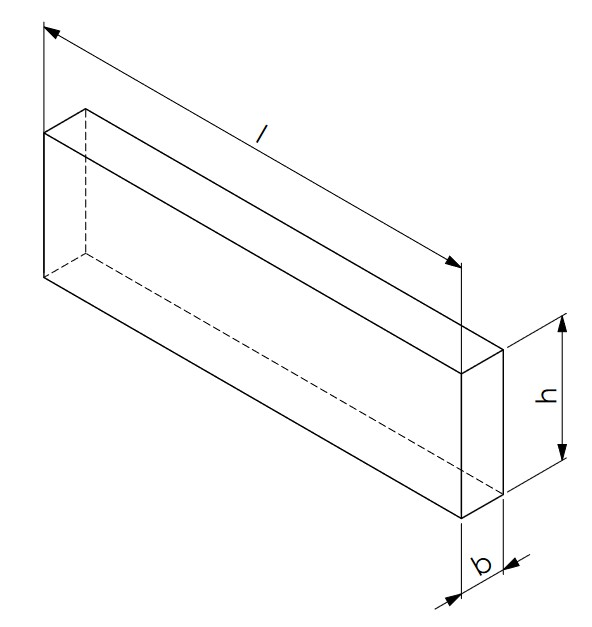
\includegraphics[width=.6\textwidth]{CAD/hall_dim.jpg}%
        \caption[Konvention der Längenbezeichnungen]{In diesem Dokument angewandte Längenbezeichnungen eines \textsc{Hall}-Plättchens mit \(h\) für
        \textit{Höhe}, \(b\) für \textit{Breite} und \(l\) für \text{Länge}.}%
        \label{fig:hall_dim}
    \end{figure}
    Damit für den spezifischen Widerstand eines Materials:
    \begin{equation}
        R = \rho \cdot \frac{l}{b h} \quad \Leftrightarrow \quad \rho = R \cdot \frac{b h}{l}%
        \label{eq:spezR}
    \end{equation}
    \subsection{\textsc{Hall}-Spannung}
        Befindet sich ein Stromdurchflossener Leiter der Breite \(b\), Höhe \(h\) und Länge \(l\) innerhalb eines externen Magnetfeldes
        \( \vec{B} \) erfahren bewegte Ladungsträger eine Kraft \(\vec{F_L}\), die orthogonal zum Magnetfeld und ihrer Bewegungsrichtung
        \( \vec{v} \) (\cref{eq:lorentz}) gerichtet ist.
        %
        \begin{equation}
            \vec{F_L} = q \cdot (\vec{v_D} \times \vec{B})%
            \label{eq:lorentz}
        \end{equation}
        %
        Die Ladungsträger können nicht über die Leiteroberfläche hinaus ausweichen und es kommt zu einer Ladungsträgerverdichtung
        auf einer Seite des Leiters und entsprechend zu einer betragsgleichen Verknappung auf der gegenüberliegenden Seite. Bei
        einer Trennung von Ladungsträgern bildet sich ein elektrisches Feld aus welches wiederum nach \cref{eq:elektrische_kraft}
        der Lorentzkraft entgegen wirkt.
        %
        \begin{equation}
            \vec{F_E} = q \vec{E}
            \label{eq:elektrische_kraft}
        \end{equation}
        %
        Im statischen Fall kommt es zu einem Gleichgewicht zwischen der elektrischen Feldkraft \(\vec{F_E}\) und der Lorentzkraft
        \(\vec{F_L}\) nach
        \begin{align}
            \vec{F_E} &= \vec{F_L} \nonumber\\
            q \cdot \vec{E} &= q \cdot (\vec{v_D} \times \vec{B}) \nonumber\\
            \frac{\vec{U_H}}{h} &= \vec{v_D} \times \vec{B} \nonumber\\
            \vec{U_H} &= h \cdot (\vec{v_D} \times \vec{B})
            \label{eq:UH1}
        \end{align}
        bzw. für den Fall, dass alle drei Vektorielle Größen jeweils orthogonal zueinander stehen:
        \begin{equation}
            U_H = h v_D B
            \label{eq:UH1ez}
        \end{equation}

        Da die Stromdichte durch die Probe mit der durchflossenen Fläche durch \(I_p = b\cdot h \cdot j\) gerade den Probenstrom ergibt
        und mit der Driftgeschwindigkeit der Ladungsträger als \(v_D=j \cdot (q\cdot n_q)\) lässt sich \cref{eq:UH1ez} überführen zu
        \begin{align}
            U_H = \frac{I_p}{b j} \cdot B \cdot \frac{j}{q n_q} = \frac{B \cdot I_p}{q n_q b}
            \label{eq:UH2}
        \end{align}
    \subsection{Magnetischer Kreis}
        %
        Das magnetische Durchflutungsgesetz bildet einen Zusammenhang zwischen der magnetischen Durchflutung \(\Theta\) und
        dem durch sie eingeschlossenen Strom \(I\) nach \cite{Halliday.2005}
        \begin{equation}
            \Theta = \oint \vec{H} \bullet d\vec{s} = I
        \end{equation}
        Im Falle einer Spule mit Eisenkern lässt sich dieser Zusammenhang vereinfacht darstellen durch
        \begin{equation}
            \Theta = N \cdot I
            \label{eq:NI}
        \end{equation}
        wobei \(N\) die Windungszahl der Spule und \(I\) der in den Windungen fließende Strom ist.

        In Analogie zum ohm'schen Gesetz gilt weiter
        \begin{equation}
            \Theta = \Phi \sum\limits_{}^{i} R_{m,i}
        \end{equation}
        mit
        \begin{equation}
            R_{m,i} = \frac{s_i}{\mu_0\mu_{r,i} A}
            \label{eq:Rm}
        \end{equation}
        Hier ist \(\Phi\) der magn. Fluss in der Einheit \(\SI{}{Wb}\), \(\mu_0\) die magn. Feldkonstante (auch Permeabilität des
        Vakuums) mit \(\approx 4\pi \cdot \SI{10^{-7}}{\newton\per\ampere\squared}\), \(\mu_r\) die (einheitenlose) materialabhängige relative
        Permeabilität und \(s\) und \(A\) die durchflutete Strecke respektive Fläche in den Einheiten \(\si{m}\) und \(\si{m\squared}\).
    %     %\section{Gleichungen und Herleitungen}
    %     %Herleitung der gegebenen Gl. aus den Grundgleichungen.